\section{Оборудование}
\subsection{Дифракция Френеля на щели}
\begin{figure}[ht!]
    \center{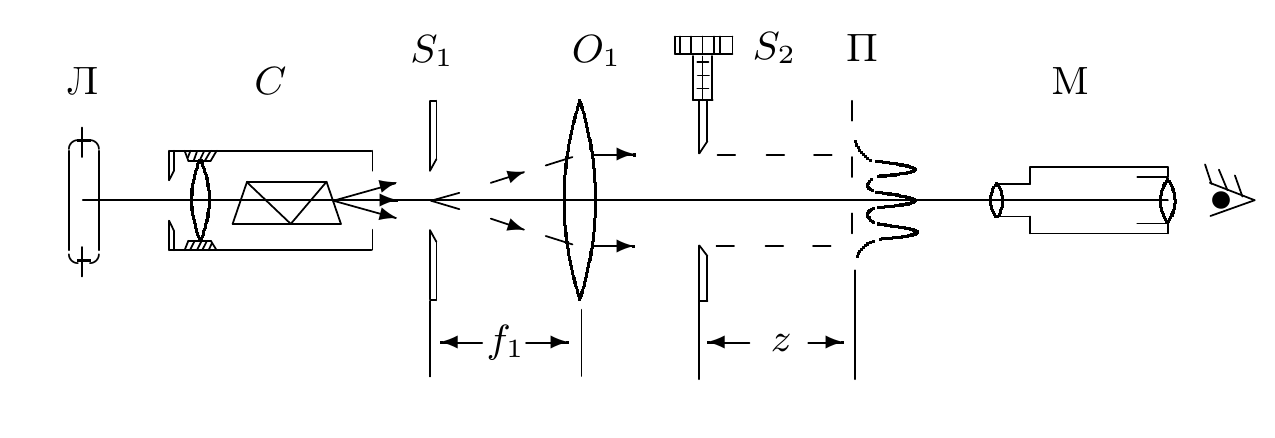
\includegraphics[width=0.8\linewidth]{../img/fren-eq.png}}
\end{figure}

Световые лучи освещают щель $S_{2}$ и испытывают на ней дифракцию. Дифракционная картина рассматривается с помощью микроскопа $M$, сфокусированного на некоторую плоскость наблюдения $\Pi$.

Щель $S_{2}$ освещается параллельным пучком монохроматического света с помощью коллиматора, образованного объективом $O_{1}$, и щелью $S_{1}$, находящейся в его фокусе. На щель $S_{1}$ сфокусировано изображение спектральной линии, выделенной из спектра ртутной лампы Л при помощи простого монохроматора $C$, в котором используется призма прямого зрения.

Распределение интенсивности света в плоскости наблюдения $\Pi$ проще всего рассчитывать с помощью зон Шустера. При освещении щели $S_{2}$ параллельным пучком лучей (плоская волна) зоны Френеля представляют собой полоски, параллельные краям щели. Результирующая амплитуда в точке наблюдения определяется суперпозицией колебаний от тех зон Френеля, которые не перекрыты створками щели. Графическое определение результирующей амплитуды производится с помощью векторной диаграммы~--- спирали Корню. Суммарная ширина $n$ зон Шустера  определяется соотношением
\[
    \xi_{n} = \sqrt{zn \lambda}
\]

Вид наблюдаемой дифракционной картины на щели шириной $b$ определяется волновым параметром:
\[
    p = \frac{\sqrt{z \lambda}}{b}  
\]

Также используют так называемое число Френеля:
\[
    C = \frac{1}{p^{2}}
\]
Это полное число открытых зон Шустера на всей ширине щели.

Дифракционная картина отсутствует вблизи щели при $p \ll 1$, а распределение интенсивности света за щелью можно приближённо получить с помощью законов геометрической оптики. Дифракционная картина в этом случае наблюдается только в узкой области на границе света и тени у краёв экрана.

При небольшом удалении от щели эти две группы дифракционных полос перемещаются практически независимо друг от друга. Каждая из этих групп образует картину дифракции Френеля на краю экрана. Распределение интенсивностипри дифракции света на краю экрана может быть найдено с помощью спирали Корню.

При дальнейшем увеличении расстояния $z$ обе системы дифракционных полос постепенно сближаются и, наконец, при $C ~ 1$ накладываются друг на друга. Распределение интенсивности в плоскости наблюдения в этом случае определяется числом зон Шустера,  укладывающихся на полуширине щели $b / 2$. Если это число равно $n$, то в поле зрения наблюдается $m = n - 1$ тёмных полос. Таким образом, по виду дифракционной картины можно оценить число зон Френеля на полуширине щели.

\subsection{Дифракция Фраунгофера на щели}
\begin{figure}[ht!]
    \center{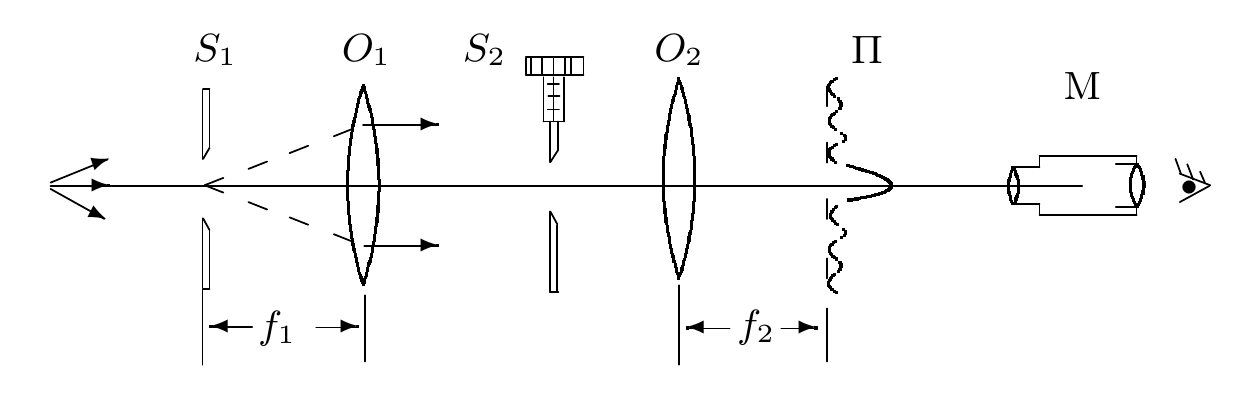
\includegraphics[width=0.8\linewidth]{../img/frau1-eq.png}}
\end{figure}

На значительном удалении от щели, когда выполнено условие $C \ll 1$, изображение щели размывается и возникает дифракционная картина, называемая дифракцией Фраунгофера.

Дифракцию Френеля и Фраунгофера можно наблюдать на одной и той же установке. Однако при обычных размерах установки дифракция Фраунгофера возникает только при очень узких щелях. Например, при $z \approx 20-40\;\text{см}$ и $\lambda \approx 5\cdot 10^{-5}\;\text{см}$ получаем $b \ll 0{,}3\;\text{мм}$. Работать с такими тонкими щелями неудобно, для наблюдения дифракции Фраунгофера к предыдущей схеме добавляется объектив $O_{2}$.

Дифракционная картина наблюдается здесь в фокальной плоскости объектива $O_{2}$. Каждому значению угла $ \theta$ соответствует в этой плоскости точка, отстоящая от оптической оси на расстоянии
\[
    x = f_{2} \tg \theta \approx f_{2} \theta
\]

Поскольку объектив не вносит дополнительной разности хода между интерферирующими лучами,  в его фокальной плоскости наблюдается неискажённая дифракционная картина Фраунгофера. Эта картина соответствует бесконечно удалённой плоскости наблюдения.

В центре поля зрения наблюдается дифракционный максимум. При малых углах $\theta$ положение минимумов определяется  соотношением
\[
    \theta_{m} = m\frac{\lambda}{b}
\]
Расстояние $x_{m}$ от тёмной полосы до оптической оси объектива $O_{2}$ пропорционально фокусному расстоянию $f_{2}$
\[
    x_{m} = m\frac{\lambda}{b}f_{2}
\]
Видно, что при малых углах минимумы эквидистантны, а расстояния $\delta x$ между минимумами обратно пропорциональны ширине $b$ щели $S_{2}$.

\subsection{Дифракция Фраунгофера на двух щелях}
Для наблюдения дифракции Фраунгофера на двух щелях в установке следует заменить щель $S_{2}$ экраном Э с двумя щелями. При этом для оценки влияния ширины входной щели на чёткость дифракционной картины вместо входной щели $S_{1}$ следует поставить щель с микрометрическим винтом. Два дифракционных изображения входной щели, одно из которых образовано лучами, прошедшими через левую, а другое~--- через правую щели, накладываются друг на друга.

\begin{figure}[ht!]
    \center{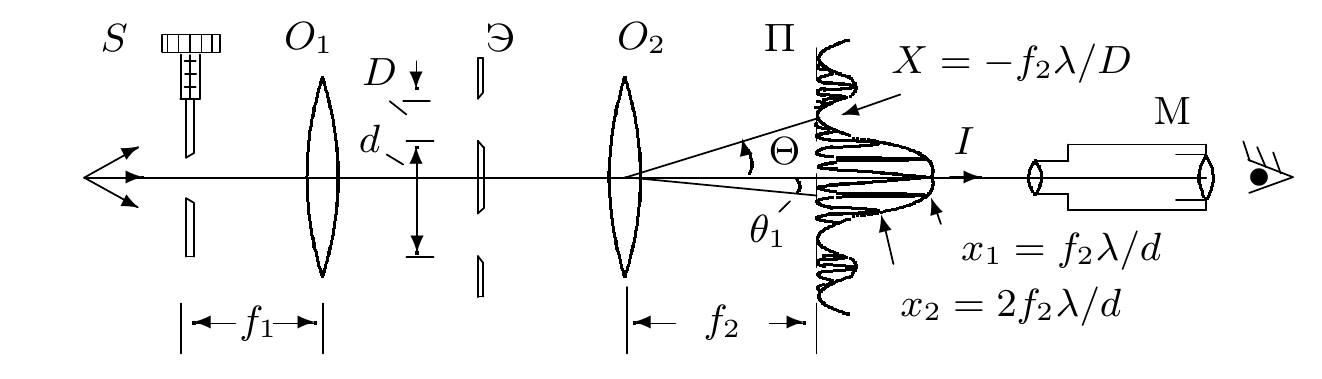
\includegraphics[width=0.8\linewidth]{../img/frau2-eq.png}}
\end{figure}

Если входная щель достаточно узка, то дифракционная картина в плоскости П подобна той, что получалась при дифракции на одной щели, однако теперь вся картина испещрена рядом дополнительных узких полос.

Как ясно из формулы, угловая координата $ \theta_{m}$ интерференционного максимума $m$-го порядка определяется соотношением
\[
    \theta_{m} = m\frac{ \lambda}{d}
\]
$d$~--- расстояние между щелями. Линейное расстояние $\delta x$ между соседними интерференционными полосами в плоскости П равно, поэтому
\[
    \delta x = f_{2} \frac{\lambda}{d}
\]
На рисунке показано распределение интенсивности в фокальной плоскости объектива $O_{2}$. Штриховой линией изображено распределение интенсивности при дифракции света на одиночной щели. Нетрудно оценить число $n$ интерференционных полос, укладывающихся в области центрального дифракционного максимума. Полная ширина главного максимума равна $2f_{2} \lambda / b$, $b$~--- ширина щели, отсюда
\[
    n = \frac{2\lambda f_{2}}{b}\frac{1}{\delta x} = \frac{2d}{b}
\]
При дифракции света на двух щелях чёткая система интерференционных полос наблюдается только при достаточно узкой ширине входной щели $S$, которую можно рассматривать как протяжённый источник света размером $b$. Для наблюдения интерференции необходимо, чтобы расстояние $d$ между щелями не превышало радиуса когерентности
\[
    d \le \frac{\lambda}{b}f_{1}
\]
Здесь $b$~--- ширина входной щели $S$ и, следовательно, $b/f_{1}$~--- её угловая ширина. Таким образом, по размытию интерференционной картины можно оценить размер источника. Этот метод используется в звёздном интерферометре при измерении угловых размеров звёзд.
